\PassOptionsToPackage{table}{xcolor}
\documentclass[aspectratio=169,24pt]{beamer}
\setbeamerfont{normal text}{size=\fontsize{14}{16}\selectfont}
\setbeamerfont{frametitle}{size=\fontsize{18}{20}\selectfont}
\setbeamerfont{title}{size=\fontsize{22}{26}\selectfont}
\makeatletter
\renewcommand\normalsize{\@setfontsize\normalsize{14}{16}}
\makeatother

% --- BUET branding ---
% Accent color requested: #ac1f25
\definecolor{buetAccent}{HTML}{AC1F25}

% --- Theme (aligned with reference/SIMD talk.tex) ---
% The theme file is beamerthemeawesome.sty. Loading it as a package matches the
% reference deck pattern and enables the Agenda + section/subsection divider slides.
\usepackage[english, secslide, coloraccent=buetAccent]{beamerthemeawesome}

% --- Packages ---
\usepackage[utf8]{inputenc}
\usepackage[T1]{fontenc}
\usepackage{lmodern}
\usepackage{graphicx}
\usepackage{booktabs}
\usepackage{array}
\usepackage{amsmath,amssymb}
\usepackage{listings}
\usepackage{xcolor}
\usepackage[backend=biber,style=authoryear]{biblatex}
\usepackage{wrapfig}
\addbibresource{aes.bib}

% --- Logo (top-right on all slides) ---
\newcommand{\buetLogoFile}{aes_files/buet-logo.png}
\newcommand{\buetLogoHeight}{0.8cm}
\setbeamertemplate{background}{%
	\begin{tikzpicture}[remember picture,overlay]
		\IfFileExists{\buetLogoFile}{%
			\node[anchor=north east,xshift=-0.35cm,yshift=-0.25cm] at (current page.north east) {%
				\includegraphics[height=\buetLogoHeight]{\buetLogoFile}%
			};%
		}{}%
	\end{tikzpicture}%
}

% --- Listings (code blocks) ---
\definecolor{codebg}{RGB}{245,246,250}
\definecolor{codekw}{RGB}{38,139,210}
\definecolor{codestr}{RGB}{211,54,130}
\definecolor{codecm}{RGB}{88,110,117}


% --- Overlay blocks palette (theme-compatible) ---
\colorlet{encComm}{buetAccent}
\colorlet{encStorage}{awesomeSlateBlue}
\colorlet{encFinance}{awesomeForestGreen}
\colorlet{encAuth}{awesomeCharcoal}
\colorlet{encVPN}{buetAccent!55!awesomeSlateBlue}
\colorlet{encDRM}{buetAccent!55!awesomeForestGreen}

\lstset{
	backgroundcolor=\color{codebg},
	basicstyle=\ttfamily\small,
	keywordstyle=\color{codekw}\bfseries,
	stringstyle=\color{codestr},
	commentstyle=\color{codecm}\itshape,
	showstringspaces=false,
	columns=fullflexible,
	frame=single,
	rulecolor=\color{black!10},
	breaklines=true,
	tabsize=2
}

\setbeamercovered{transparent=20}

% --- Metadata ---
\title[Advanced Encryption Standard]{AES encryption}
\subtitle{Advanced Encryption Standard}
\author{CSE 22 B1 Group 4}
\email{2205070@ugrad.cse.buet.ac.bd 2205079@ugrad.cse.buet.ac.bd 2205068@ugrad.cse.buet.ac.bd}
\institute{Department of Computer Science}
\uni{Bangladesh University of Engineering and Technology}
\location{Dhaka, Bangladesh}
\background{aes_files/cover_bg.jpeg}
\date\today

\begin{document}

% Theme defines \maketitle to include an Agenda slide (unless [notoc]).
\maketitle

\section{Introduction}

\begin{frame}{Introduction}
	\begin{wide}\only<1>{\begin{itemize}
		\item Advanced Encryption Standard (AES) is the world's most widely used encryption algorithm
		\item Adopted by US government in 2001 to protect sensitive information
		\item Replaced the aging Data Encryption Standard (DES)
		\item Used in everything from secure web browsing (HTTPS) to encrypted messaging and data storage
		\item Foundation of modern digital security
	\end{itemize}}
	
	\only<2>{\textbf{Why AES Matters:} \\
		AES secures billions of online transactions, communications, and data storage operations every day. By doing so, it helps create a safer digital world where privacy and trust are possible.}
	\end{wide}
\end{frame}

\section{Understanding Encryption}

\begin{frame}{What is Encryption?}
	\begin{wide}
	\only<1->{
		\begin{block}{\textbf{Definition: }}
			Encryption converts readable data (\textit{plaintext}) into unreadable data (\textit{ciphertext}) using an algorithm and a key.
		\end{block}
	}
	\only<2->{\begin{columns}[T,onlytextwidth]
		\column{0.55\textwidth}
			
			\vspace{0.5em}
			\begin{itemize}
				\item Hides information as secret code
				\item Only the right key can decrypt
			\end{itemize}
		
		\column{0.45\textwidth}
			\begin{figure}
				\centering
				\begin{tikzpicture}[scale=0.8, transform shape]
					% Plaintext box
					\node[squarenode, fill=awesomeForestGreen!20, text width=3cm, align=center] (plain) at (0,0) {Plaintext\\\small ``Hello World''};
					
					% Encryption arrow
					\draw[arrow] (plain) -- node[right, text width=1.8cm, align=center] {\small Encryption\\Key}
						 node[left, text width=2.2cm, align=center] {\small Encryption\\Algorithm} (0,-2);
					
					% Ciphertext box
					\node[squarenode, fill=awesomeSlateBlue!20, text width=3cm, align=center] (cipher) at (0,-2.5) {Ciphertext\\\small ``3k7m9x2...''};
				\end{tikzpicture}
				\caption{Encryption process}
			\end{figure}
	\end{columns}}
	\end{wide}
\end{frame}

\begin{frame}{Why Encryption Matters}
	\begin{wide}
	\only<1-3>{\begin{itemize}
		\onslide<1-3>{\item \textbf{Confidentiality}: Stolen data stays unreadable without the key.}
		\onslide<2-3>{\item \textbf{Privacy}: Protects messages, personal data, and transactions from eavesdropping.}
		\onslide<3>{\item \textbf{Compliance}: Needed for standards/laws (e.g., GDPR, HIPAA, PCI-DSS).}
	\end{itemize}}
	\only<4-5>{\begin{itemize}
		\onslide<4-5>{\item \textbf{Threat defense}: Helps against breaches, MITM, and ransomware fallout.}
		\onslide<5>{\item \textbf{Trust \& integrity}: Reduces tampering risk and increases confidence.}
	\end{itemize}}
	\end{wide}
\end{frame}

\begin{frame}{Application of Encryption}
	\begin{wide}
		\vspace{-1em}
	\begin{columns}[T,onlytextwidth]
		\column{0.45\textwidth}
		\onslide<1->{%
			\begin{beamerbox}{encComm}{Secure Communications}
				\small HTTPS, encrypted messaging (Signal/WhatsApp)
			\end{beamerbox}
		}

		% \vspace{0.1em}
		\onslide<3->{%
			\begin{beamerbox}{encFinance}{Financial Transactions}
				\small Online banking, card payments
			\end{beamerbox}
		}

		\onslide<5->{%
			\begin{beamerbox}{encVPN}{Virtual Private Networks}
				\small Encrypted traffic for privacy/security
			\end{beamerbox}
		}

		\column{0.45\textwidth}
		\onslide<2->{%
			\begin{beamerbox}{encStorage}{Data Storage}
				\small Disk + cloud encryption
			\end{beamerbox}
		}

		\vspace{0.1em}
		\onslide<4->{%
			\begin{beamerbox}{encAuth}{Authentication}
				\small Password hashing, secure tokens
			\end{beamerbox}
		}

		\onslide<6->{%
			\begin{beamerbox}{encDRM}{Digital Rights}
				\small Prevents unauthorized copying/use
			\end{beamerbox}
		}
	\end{columns}
	
	\end{wide}
\end{frame}

\section{Characteristics of Good Encryption}

\begin{frame}{Need for understanding good encryption criteria}
	\begin{wide}
	Before AES, it helps to know what makes an encryption standard \textit{good}. These criteria explain why AES is designed the way it is.
	\end{wide}
\end{frame}

% Overview slide with all main points enumerated
\begin{frame}{Criteria for Good Encryption}
	\begin{wide}
	\centering
	\begin{tikzpicture}[scale=0.95, transform shape]
		\tikzset{critbox/.style={
			roundednode,
			rnd,
			lw,
			minimum width=4.7cm,
			minimum height=1.25cm,
			text width=4.3cm,
			align=center,
			font=\small\bfseries
		}}

		% Row 1 (3 boxes)
		\node[critbox, fill=buetAccent!88, text=white, visible on=<1->] at (-5.0, 1.0)
			{Public, well-specified design};

		\node[critbox, fill=awesomeSlateBlue!92, text=white, visible on=<2->] at (0, 1.0)
			{Strong design principles\\[-1pt]\scriptsize (Shannon's Principles)};

		\node[critbox, fill=awesomeForestGreen!90, text=white, visible on=<3->] at (5.0, 1.0)
			{Large key space and\\dependable key handling};

		% Row 2 (2 boxes)
		\node[critbox, fill=awesomeCharcoal!92, text=white, visible on=<4->] at (-2.5, -1.0)
			{Resistance to known\\attack classes};

		\node[critbox, fill=buetAccent!60!awesomeSlateBlue!85, text=white, visible on=<5->] at (2.5, -1.0)
			{Efficiency in software\\and hardware};
	\end{tikzpicture}
	\end{wide}
\end{frame}

% Slide 1: Public Design

\subsection*{Public, Well-Specified Design}

\begin{frame}{Public, Well-Specified Design}
	\begin{wide}
	A good standard is openly documented (algorithm, parameters, test vectors) so experts can review it, implement it consistently, and find flaws early.
	
	\vspace{1em}
	\begin{block}{\textbf{Key Point}}
		Transparency enables peer review and builds trust.
	\end{block}
	\end{wide}
\end{frame}

% Slide 2: Strong Design Principles Overview
% Slide 2: Strong Design Principles Overview (fixed; no wrapfigure)

\subsection*{Strong Design Principles}

\begin{frame}{Strong Design Principles}
	\begin{wide}
	\framesubtitle{Shannon's Principles}

	\begin{columns}[T,onlytextwidth]
		\column{0.65\textwidth}
			
			\vspace{1em}
			A robust encryption standard follows Shannon's core principles:

			\vspace{0.6em}
			\begin{itemize}
				\item Confusion
				\item Diffusion
				\item Adequate Key Size
			\end{itemize}





		\hfill
		\column{0.30\textwidth}
			\begin{figure}
				\centering
				\includegraphics[width=\linewidth]{aes_files/Shannon.jpg}
				\caption{Claude E. Shannon}
				\label{fig:Shannon}
			\end{figure}
	\end{columns}
\end{wide}
\end{frame}


% Uses TikZ styles/libraries provided by your theme (roundednode, arrow, visible on, positioning, etc.). [file:17][file:18]

% Slide 3: Confusion (2-column, vertical diagram on right)
\begin{frame}{Shannon's Principle: Confusion}
	\begin{wide}
	\begin{columns}[T,onlytextwidth]
		\column{0.5\textwidth}
			Make the plaintext\textendash ciphertext\textendash key relationship hard to predict.
			
			\vspace{0.5em}
			\begin{exampleblock}{\textbf{Example}}
				Non-linear substitutions (S-boxes) make key recovery from patterns difficult.
			\end{exampleblock}
		
		\column{0.5\textwidth}
			\centering
			\begin{tikzpicture}[scale=0.95, transform shape]
				% Nodes (vertical layout)
				\node[roundednode, fill=awesomeSlateBlue!20, minimum width=2.6cm] (pt) at (0,4.1) {\small Plaintext};
				\node[roundednode, fill=awesomeSlateBlue!20, minimum width=2.6cm] (k)  at (3,4.1) {\small Key};

				% IMPORTANT: align=center avoids the "Not allowed in LR mode" error when using \\ in node text.
				\node[roundednode, align=center, fill=buetAccent!70, text=white,
					  minimum width=3.0cm, minimum height=1.25cm] (sbox) at (0,1.7)
					  {\textbf{S-Box}\\[-1pt]\scriptsize Non-linear mapping};

				\node[roundednode, fill=awesomeForestGreen!35, minimum width=2.6cm] (ct) at (0,0.2) {\small Ciphertext};

				% Arrows (vertical flow)
				\draw[arrow] (pt) -- (sbox);
				\draw[arrow] (k)  -- (sbox);
				\draw[arrow] (sbox) -- (ct);

				% Annotation (avoid \\ inside \textcolor; use align + node color instead)
				\node[roundednode, align=left, fill=white, draw=buetAccent, text=buetAccent,
					  font=\tiny, inner sep=2.2pt] at (3.0,1.7)
					  {\shortstack[l]{Goal:\\Hide key--ciphertext\\relationships}};
			\end{tikzpicture}
	\end{columns}
		\end{wide}
\end{frame}


% Slide 4: Diffusion (2-column, animated overlay diagram on right)
\begin{frame}{Shannon's Principle: Diffusion}
	\begin{wide}
	\begin{columns}[T,onlytextwidth]
		\column{0.5\textwidth}
			Small input changes should spread widely in the output.
			
			\vspace{1em}
			\begin{exampleblock}{\textbf{Avalanche Effect}}
				Flip 1 plaintext bit \textrightarrow\ about half the ciphertext bits change.
			\end{exampleblock}
		
		\column{0.5\textwidth}
			\centering
			\begin{tikzpicture}[scale=0.92, transform shape]
				% --- Base diagram (always visible): plaintext, diffusion layer, ciphertext; NO arrows ---
				\node[font=\scriptsize, anchor=east] at (-0.35,3.60) {Plaintext:};
				\foreach \i/\b in {0/1,1/0,2/1,3/0,4/1,5/1,6/0,7/1} {
					\node[circle, draw=black!30, fill=white, inner sep=2pt, font=\tiny]
						(in\i) at (\i*0.42,3.60) {\b};
				}

				\node[roundednode, fill=buetAccent!70, text=white,
					  minimum width=3.2cm, minimum height=0.75cm] (diff) at (1.47,2.45)
					  {\small Diffusion Layer};

				\node[font=\scriptsize, anchor=east] at (-0.35,1.15) {Ciphertext:};
				\foreach \i/\b in {0/0,1/1,2/1,3/0,4/0,5/1,6/1,7/0} {
					\node[circle, draw=black!30, fill=white, inner sep=2pt, font=\tiny]
						(out\i) at (\i*0.42,1.15) {\b};
				}

				% --- Overlay (appears on 2nd click): one bit flip + many output flips + arrows ---
				% Bit flip in plaintext (choose bit 3 here: 0 -> 1)
				\node[circle, draw=buetAccent, fill=buetAccent!25, line width=1.0pt,
					  inner sep=2pt, font=\tiny, visible on=<2->] (in3flip)
					  at (3*0.42,3.60) {1};

				% Multiple flips in ciphertext (example flips)
				\node[circle, draw=awesomeForestGreen, fill=awesomeForestGreen!35, line width=1.0pt,
					  inner sep=2pt, font=\tiny, visible on=<2->] (out0flip)
					  at (0*0.42,1.15) {1};

				\node[circle, draw=awesomeForestGreen, fill=awesomeForestGreen!35, line width=1.0pt,
					  inner sep=2pt, font=\tiny, visible on=<2->] (out2flip)
					  at (2*0.42,1.15) {0};

				\node[circle, draw=awesomeForestGreen, fill=awesomeForestGreen!35, line width=1.0pt,
					  inner sep=2pt, font=\tiny, visible on=<2->] (out4flip)
					  at (4*0.42,1.15) {1};

				\node[circle, draw=awesomeForestGreen, fill=awesomeForestGreen!35, line width=1.0pt,
					  inner sep=2pt, font=\tiny, visible on=<2->] (out5flip)
					  at (5*0.42,1.15) {0};

				\node[circle, draw=awesomeForestGreen, fill=awesomeForestGreen!35, line width=1.0pt,
					  inner sep=2pt, font=\tiny, visible on=<2->] (out7flip)
					  at (7*0.42,1.15) {1};

				% Arrows from flipped plaintext bit to flipped ciphertext bits
				\draw[arrow, buetAccent, line width=0.7pt, visible on=<2->]
					(in3flip) to[out=-90, in=90] (out0flip);
				\draw[arrow, buetAccent, line width=0.7pt, visible on=<2->]
					(in3flip) to[out=-90, in=90] (out2flip);
				\draw[arrow, buetAccent, line width=0.7pt, visible on=<2->]
					(in3flip) to[out=-90, in=90] (out4flip);
				\draw[arrow, buetAccent, line width=0.7pt, visible on=<2->]
					(in3flip) to[out=-90, in=90] (out5flip);
				\draw[arrow, buetAccent, line width=0.7pt, visible on=<2->]
					(in3flip) to[out=-90, in=90] (out7flip);

				% Caption (appears with overlay)
				\node[font=\tiny, text=buetAccent, visible on=<2->] at (1.47,0.40)
					{1 bit flip $\rightarrow$ many bits change};
			\end{tikzpicture}
	\end{columns}
		\end{wide}
\end{frame}

% Slide 5: Key Size
\begin{frame}{Shannon's Principle: Key Size}
	\begin{wide}
	Keys must be large enough to make brute-force search impractical.
	
	\vspace{1em}
	\begin{block}{\textbf{Modern Standards}}
		\begin{itemize}
			\item 128-bit: $2^{128}$ keys
			\item 256-bit: $2^{256}$ keys
			\item Exhaustive search is infeasible today
		\end{itemize}
	\end{block}
	\end{wide}
\end{frame}

% Slide 6: Large Key Space

\subsection*{Large Key Space \& Key Handling}

\begin{frame}{Large Key Space \& Key Handling}
	\begin{wide}
	Beyond "big keys," a good standard defines safe key formats/schedules and practical guidance (generate, store, rotate) to avoid weak or predictable keys.
	
	\vspace{1em}
	\begin{alertblock}{\textbf{Warning}}
		Poor key management breaks even strong algorithms.
	\end{alertblock}
	\end{wide}
\end{frame}

\subsection*{Resistance to Attacks}

% Slide 7: Resistance to Attacks
\begin{frame}{Resistance to Known Attack Classes}
	\begin{wide}
	A strong standard is tested against known cryptanalysis and keeps a practical security margin.
	
	\vspace{1em}
	\begin{itemize}
		\item Differential cryptanalysis
		\item Linear cryptanalysis
		\item Side-channel attacks
		\item Brute-force attacks
	\end{itemize}
	\end{wide}
\end{frame}

% Slide 8: Efficiency

\subsection*{Efficiency in Software \& Hardware}

\begin{frame}{Efficiency in Software \& Hardware}
	\begin{wide}
	If encryption is too slow, people disable or misuse it; a good standard is fast on common devices.
	
	\vspace{1em}
	\begin{block}{\textbf{Practical Requirements}}
		\begin{itemize}
			\item Real-time throughput (e.g., streaming)
			\item Low power on mobile
			\item Hardware acceleration support
		\end{itemize}
	\end{block}
	\end{wide}
\end{frame}

% Add these frames after the existing sections in your presentation

% \section{History of AES}

% \begin{frame}{The Need for a New Standard}
% 	\begin{columns}[T,onlytextwidth]
% 		\column{0.6\textwidth}
% 			\begin{itemize}
% 				\item Data Encryption Standard (DES) published in 1977
% 				\item By late 1990s, DES became vulnerable to brute-force attacks
% 				\item 1997: Deep Crack machine broke DES in 56 hours
% 				\item Need for stronger encryption became critical
% 			\end{itemize}
		
% 		\hfill
% 		\column{0.3\textwidth}
% 			\begin{figure}
% 				\centering
% 				\includegraphics[width=0.9\linewidth]{aes_files/des_cracker.jpg}
% 				\caption{Deep Crack DES cracking machine}
% 			\end{figure}
% 	\end{columns}
% \end{frame}

% \begin{frame}{NIST Announces AES Competition}
% 	\begin{columns}[T,onlytextwidth]
% 		\column{0.65\textwidth}
% 			\begin{itemize}
% 				\item January 2, 1997: NIST announced effort to develop AES
% 				\item September 12, 1997: Formal call for algorithms
% 				\item Requirements:
% 				\begin{itemize}
% 					\item Unclassified, publicly disclosed
% 					\item Symmetric key block cipher
% 					\item 128-bit block size
% 					\item Support 128, 192, and 256-bit keys
% 					\item Royalty-free worldwide
% 				\end{itemize}
% 			\end{itemize}
		
% 		\hfill
% 		\column{0.30\textwidth}
% 			\begin{figure}
% 				\centering
% 				\includegraphics[width=0.9\linewidth]{aes_files/nist_logo.jpg}
% 				\caption{National Institute of Standards and Technology (NIST)}
% 			\end{figure}
% 	\end{columns}
% \end{frame}

% \begin{frame}{The Competition Process}
% 	\begin{itemize}
% 		\item \textbf{1998}: 15 candidate algorithms submitted from around the world
% 		\item \textbf{August 1999}: NIST selected 5 finalists:
% 		\begin{itemize}
% 			\item MARS (IBM)
% 			\item RC6 (RSA Security)
% 			\item Rijndael (Joan Daemen \& Vincent Rijmen)
% 			\item Serpent (Ross Anderson, Eli Biham, Lars Knudsen)
% 			\item Twofish (Bruce Schneier et al.)
% 		\end{itemize}
% 		\item Extensive public analysis and evaluation
% 		\item Open, transparent process praised by cryptographic community
% 	\end{itemize}
% \end{frame}

% \begin{frame}{The Creators of Rijndael}
% 	\begin{columns}[T,onlytextwidth]
% 		\column{0.4\textwidth}
% 			\begin{figure}
% 				\centering
% 				\includegraphics[width=0.3\linewidth]{aes_files/joan_daeman.png}
% 				\caption{Joan Daemen}
% 			\end{figure}
% 			\begin{itemize}
% 				\item Belgian cryptographer
% 				\item Born 1965
% 				\item Professor at Radboud University
% 			\end{itemize}
		
% 			\hfill
% 		\column{0.4\textwidth}
% 			\begin{figure}
% 				\centering
% 				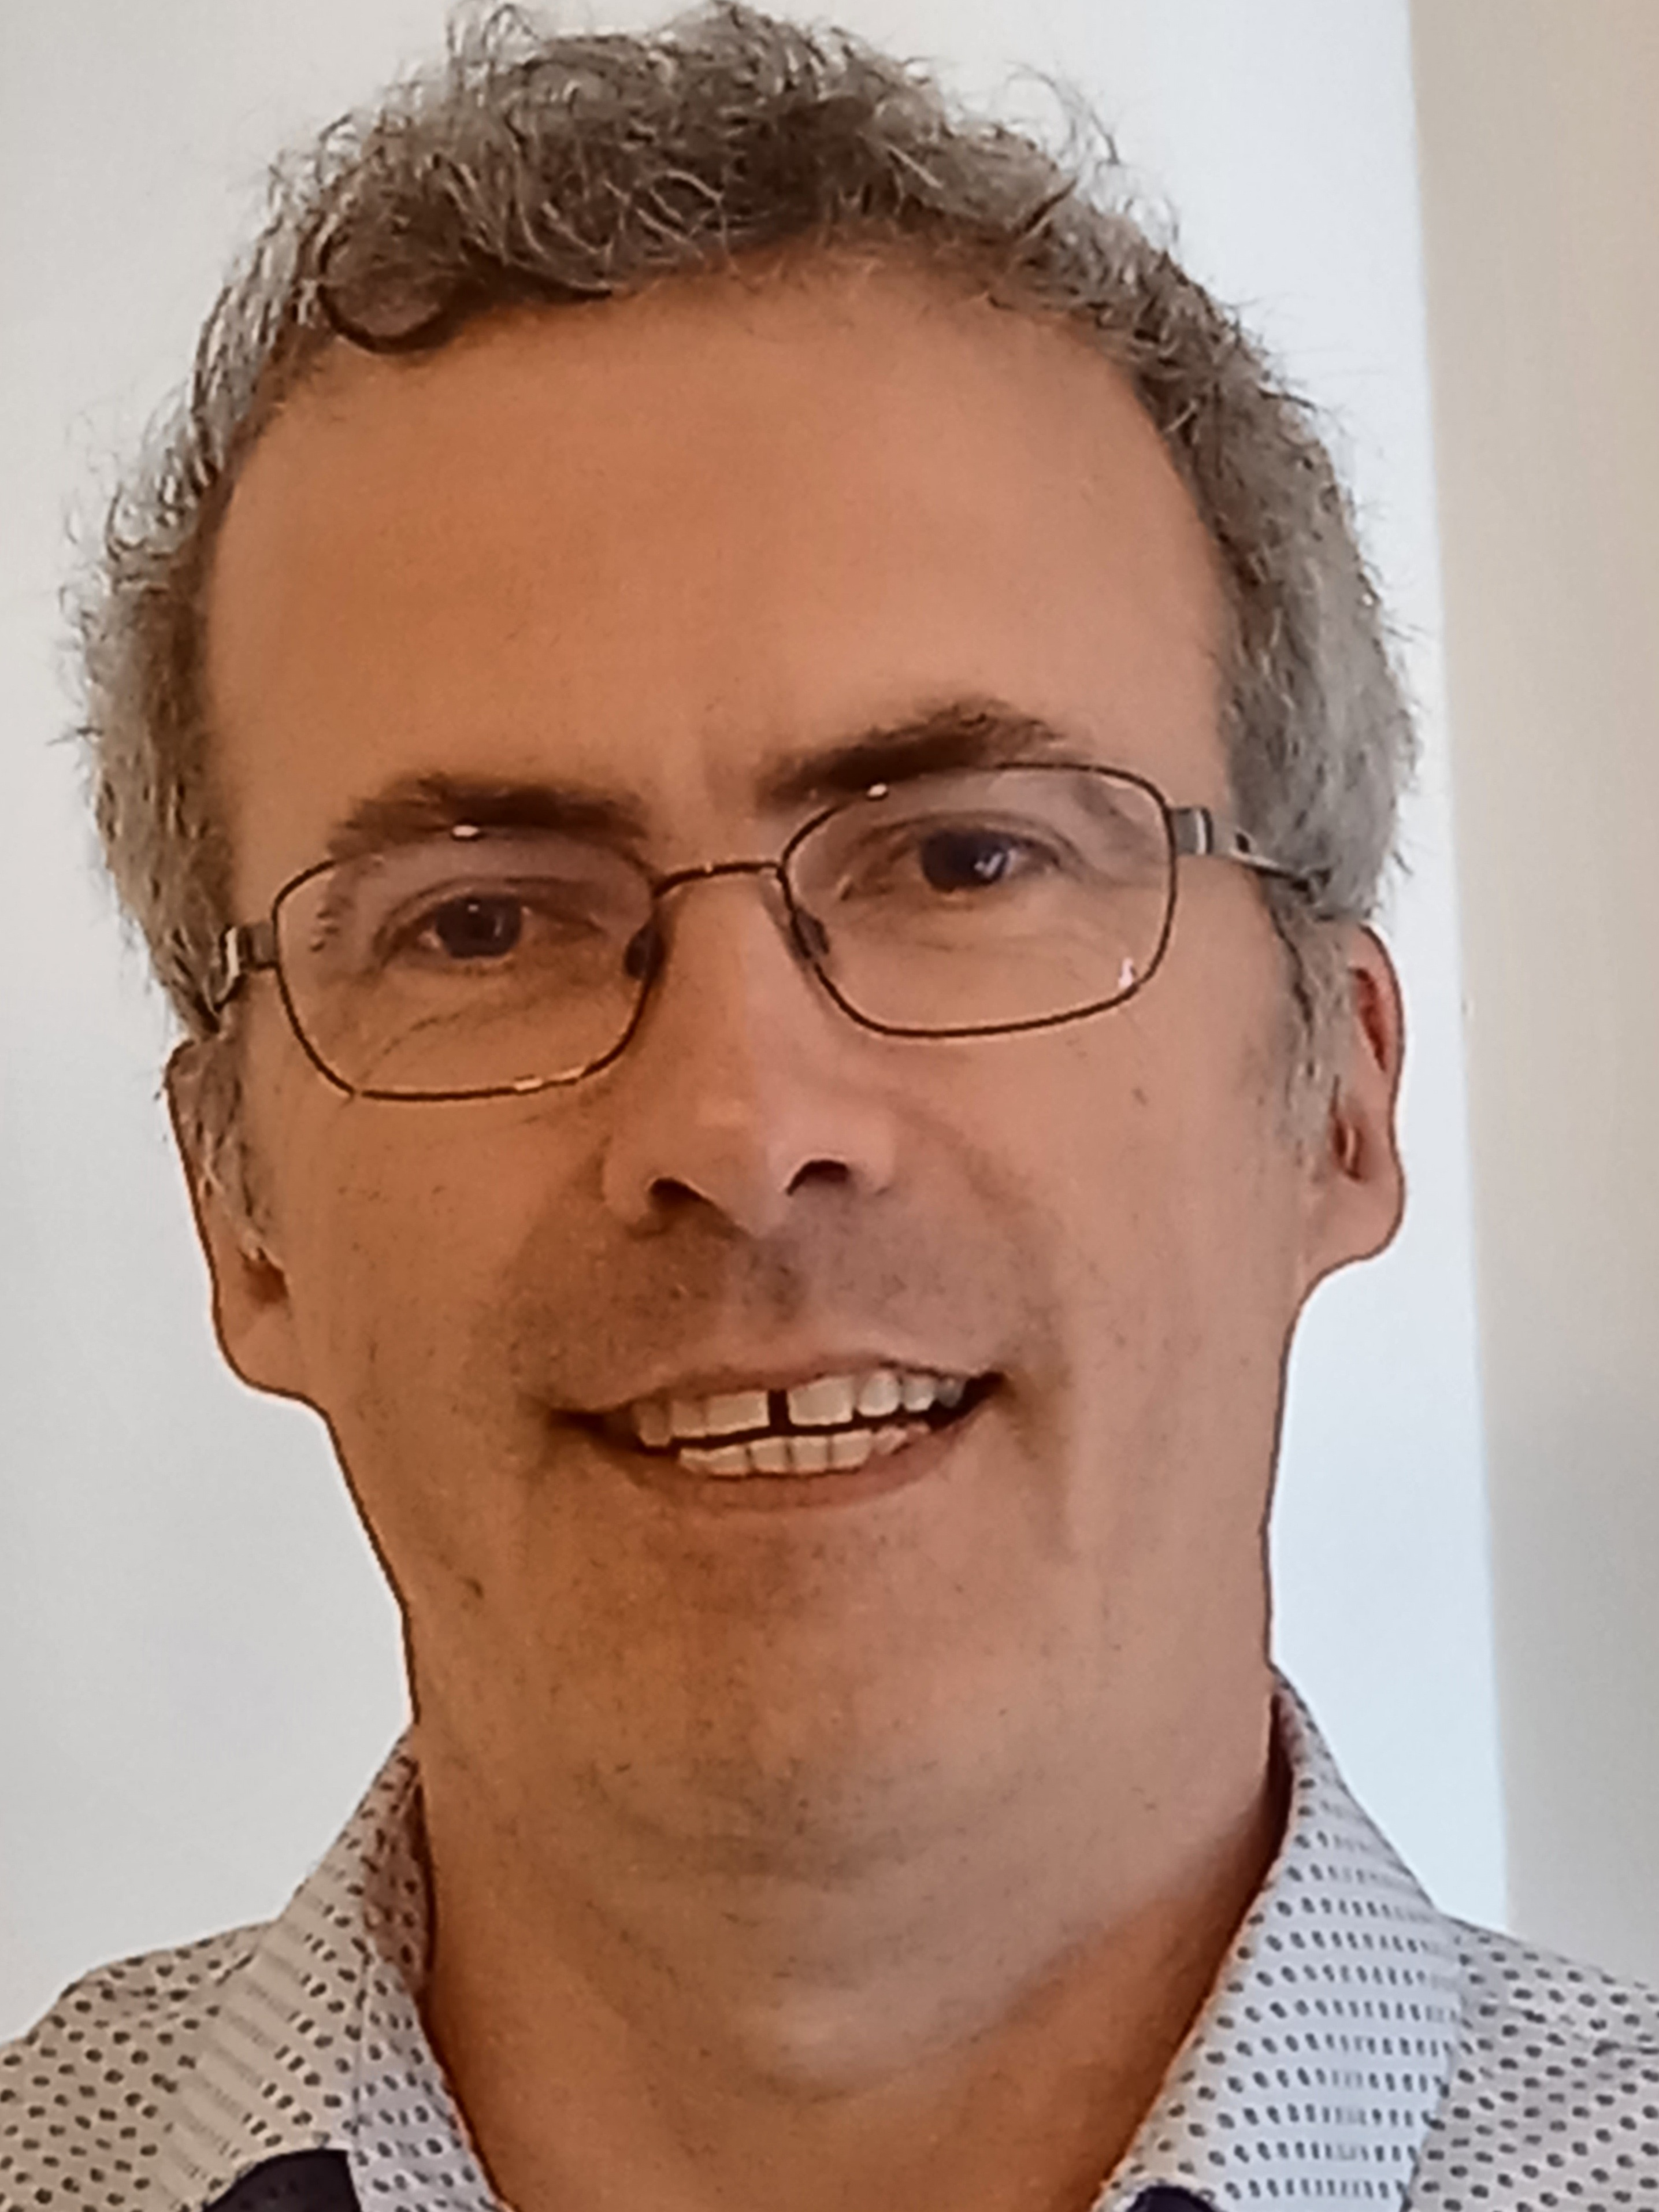
\includegraphics[width=0.3\linewidth]{aes_files/vincent_rijmen.png}
% 				\caption{Vincent Rijmen}
% 			\end{figure}
% 			\begin{itemize}
% 				\item Belgian cryptographer
% 				\item Co-designed Rijndael cipher
% 				\item Algorithm name combines their surnames
% 			\end{itemize}
% 	\end{columns}
% \end{frame}

% \begin{frame}{Rijndael Wins the Competition}
% 	\begin{itemize}
% 		\item \textbf{October 2, 2000}: NIST announced Rijndael as winner
% 		\item Selected for:
% 			\begin{itemize}
% 				\item Robust security
% 				\item Efficiency in software and hardware
% 				\item Flexibility in key and block sizes
% 				\item Superior performance characteristics
% 			\end{itemize}
% 		\item \textbf{November 26, 2001}: Published as FIPS 197
% 	\end{itemize}
% \end{frame}

% \begin{frame}{Timeline Summary}
% 	\begin{table}
% 		\centering
% 		\begin{tabular}{@{}ll@{}}
% 			\toprule
% 			\textbf{Date} & \textbf{Event} \\
% 			\midrule
% 			1977 & DES published \\
% 			Jan 2, 1997 & NIST announces AES initiative \\
% 			Sep 12, 1997 & Formal call for algorithms \\
% 			1998 & 15 candidates submitted \\
% 			Aug 1999 & 5 finalists selected \\
% 			Oct 2, 2000 & Rijndael chosen as AES \\
% 			Nov 26, 2001 & AES published as FIPS 197 \\
% 			\bottomrule
% 		\end{tabular}
% 		\caption{Key dates in AES development}
% 	\end{table}
% \end{frame}

\section{Rijndael Algorithm}

\subsection*{Overview}

\begin{frame}{What is Rijndael?}
	\begin{wide}
	\begin{itemize}
		\item \textbf{Rijndael} is the algorithm underlying AES (Advanced Encryption Standard).
		\item Designed by Joan Daemen and Vincent Rijmen.
		\item A symmetric block cipher with variable block and key sizes.
		\item Selected as the AES standard by NIST in 2001.
	\end{itemize}

	\vspace{0.5em}
	\begin{alertblock}{\textbf{Key Characteristics}}
		Block size: 128 bits | Key size: 128, 192, or 256 bits
	\end{alertblock}
	\end{wide}
\end{frame}

\begin{frame}{AES Core Operations}
	\begin{wide}
    \begin{itemize}
        \item \textcolor{buetAccent}{\textbf{Key Expansion}}
        \item SubBytes
        \item ShiftRows
        \item MixColumns
        \item AddRoundKey
    \end{itemize}
	\end{wide}
\end{frame}

\subsection*{Key Expansion}

\begin{frame}{Key Expansion Process}
	\begin{wide}
	
	\begin{itemize}
		\item Expands cipher key into round keys.
		\item Number of round keys depends on key size:
		\begin{itemize}
			\item \Large{128-bit key: 11 round keys}
			\item \Large{192-bit key: 13 round keys}
			\item \Large{256-bit key: 15 round keys}
		\end{itemize}
		\item Uses \textbf{RotWord}, \textbf{SubWord}, and \textbf{Rcon} functions.
	\end{itemize}
	\begin{block}{\textbf{Rcon Values}}
		Round-dependent constants used in key schedule to add asymmetry.
	\end{block}
	\end{wide}
\end{frame}

\begin{frame}[fragile]{Simplified Key Expansion Algorithm}
	\begin{wide}
	\begin{lstlisting}[language=Python]
def key_expansion(key, rounds):
    w = []
    # Copy original key
    for i in range(4):
        w.append(key[i])
    
    # Generate round keys
    for i in range(4, 4*(rounds+1)):
        temp = w[i-1]
        if i % 4 == 0:
            temp = SubWord(RotWord(temp))
            temp ^= Rcon[i//4]
        w.append(w[i-4] ^ temp)
    return w
	\end{lstlisting}
	\end{wide}
\end{frame}

\begin{frame}{Key Expansion: Detailed Process}
	\begin{wide}
    \only<1>{\begin{columns}[T,onlytextwidth]
        \column{0.6\textwidth}
            \textbf{The Objective}
            \begin{itemize}
                \item Transform the \textit{Cipher Key} into a \textit{Key Schedule}.
                \item AES-128 requires \textbf{176 bytes} (11 keys of 16 bytes each).
            \end{itemize}

        \column{0.4\textwidth}
            \begin{figure}
                \centering
                \IfFileExists{aes_files/key_expansion.png}{%
                    \includegraphics[width=\linewidth]{aes_files/key_expansion.png}
                }{%
                    \fbox{\parbox[c][5cm][c]{0.9\linewidth}{\centering \small Image Placeholder:\\ Key Schedule\\ Diagram}}
                }
                \caption{Recursive Key Generation}
            \end{figure}
    \end{columns}}
	\only<2->{
		\vspace{0.5em}
            \textbf{The Core Transformation ($g$ function)}
            \begin{enumerate}
                \onslide<2->\item {\textbf{RotWord}: One-byte left circular shift.}
                \onslide<3->\item {\textbf{SubWord}: Non-linear byte substitution using S-Box.}
                \onslide<4->\item {\textbf{Rcon}: XOR with a round-dependent constant to eliminate patterns.}
            \end{enumerate}
			\onslide<2->{\begin{block}{\textbf{Diffusion}}
                A change in one bit of the original key affects multiple bits in all subsequent round keys.
            \end{block}}
	}
	\end{wide}
\end{frame}

\begin{frame}{Key Expansion}
	\begin{wide}
    \centering
    \Large
    \vspace{0.1cm}

    % The Binary String
    \texttt{10100111  00111011}

    
    
    % The Curly Brackets (Revealed on click 2)
    \uncover<2->{
        $\underbrace{\hspace{1.8cm}}_{W_0} \quad \underbrace{\hspace{1.8cm}}_{W_1}$
    }

    \vspace{0.5cm}

    % The Hex Translation (Revealed on click 3)
    \uncover<3->{
        \begin{columns}[c]
            \column{0.5\textwidth}
                \centering
                \textcolor{buetAccent}{\texttt{0x A7}}
            \column{0.5\textwidth}
                \centering
                \textcolor{buetAccent}{\texttt{0x 3B}}
        \end{columns}
    }

    \vfill
    \begin{itemize}
        \item<1-> Initial state in binary (16 bits total).
        \item<2-> Grouped into two 8-bit \textbf{words} ($W_0$ and $W_1$).
        \item<3-> Converted to Hexadecimal for the Expansion algorithm.
    \end{itemize}
	\end{wide}
\end{frame}

\begin{frame}{Key Expansion: Detailed Process}
	\begin{wide}
    \begin{block}{\textbf{Initial Key: \texttt{0xA73B}}}
        Split into words: $W_0 = \text{A7}$, $W_1 = \text{3B}$
    \end{block}

    \textbf{Step 1: Generate $W_2$}
            \begin{itemize}
                \onslide<1->{\item \textbf{RotWord}($W_1$): $3B \rightarrow B3$}
                \onslide<2->{\item \textbf{SubWord}: $B3 \rightarrow 17$ (via S-Box)}
                \onslide<3->{\item \textbf{Rcon}: $17 \oplus 80 = 97$}
                \onslide<4->{\item \textbf{Result}: $W_0 \oplus 97 = \mathbf{30}$}
            \end{itemize}
		\end{wide}
\end{frame}

\begin{frame}{Key Expansion: Detailed Process}
	\begin{wide}

    \textbf{Step 2: Generate $W_3$}
            \begin{itemize}
                \onslide<1->{\item \textbf{Logic}: $W_2 \oplus W_1$}
                \onslide<2->{\item \textbf{Calculation}: $30 \oplus 3B$}
                \onslide<3->{\item \textbf{Result}: $\mathbf{0B}$}
            \end{itemize}
            
            \vspace{1em}
            \onslide<3->{\begin{alertblock}{\textbf{Round Key 1}}
                $W_2W_3 = \mathbf{0x300B}$
            \end{alertblock}

    \vspace{1em}
    \centering
    \textit{This process repeats using Round Key 1 to generate Round Key 2, and so on, until all round keys are derived.}}
	\end{wide}
\end{frame}

\begin{frame}{Key Expansion: \\ Step-by-Step Visualization}
	\begin{wide}
	\centering
    \vspace{-1.3em}

\begin{tikzpicture}[
		scale=1.05,
		transform shape,
		node distance=0.8cm,
		box/.style={rectangle, draw=black, lw, minimum width=1cm, minimum height=0.6cm, font=\ttfamily\scriptsize},
		label/.style={font=\tiny, text=darkgray},
		arrow/.style={-Latex, line width=0.75pt, text=black},
		operation/.style={rectangle, rounded corners, fill=buetAccent!20, draw=buetAccent, lw, minimum width=1.2cm, minimum height=0.5cm, font=\tiny, align=center},
		result/.style={rectangle, rounded corners, fill=awesomeForestGreen!30, draw=awesomeForestGreen, lw, minimum width=1cm, minimum height=0.6cm, font=\ttfamily\scriptsize}
	]

	% -------------------------
	% Line 1: Input + RotWord + SubWord
	% -------------------------
	\node[box, visible on=<1->] (w0) {A7};
	\node[label, above=0.03cm of w0, visible on=<1->] {$W_0$};

	\node[box, right=0.35cm of w0, visible on=<1->] (w1) {3B};
	\node[label, above=0.03cm of w1, visible on=<1->] {$W_1$};

	\node[operation, right=0.8cm of w1, visible on=<2->] (rotop) {RotWord\\{\tiny shift}};
	\node[box, right=0.35cm of rotop, visible on=<2->] (rot) {B3};
	\draw[arrow, visible on=<2->] (w1) -- (rotop);
	\draw[arrow, visible on=<2->] (rotop) -- (rot);

	\node[operation, right=0.8cm of rot, visible on=<3->] (subop) {SubWord\\{\tiny S-Box}};
	\node[box, right=0.35cm of subop, visible on=<3->] (sub) {17};
	\draw[arrow, visible on=<3->] (rot) -- (subop);
	\draw[arrow, visible on=<3->] (subop) -- (sub);

	% -------------------------
	% Line 2: Rcon XOR + W2 generation
	% -------------------------
	\node[box, below=1.2cm of w0, visible on=<4->] (sub2) {17};
	\node[label, above=0.03cm of sub2, visible on=<4->] {SubWord};

	\node[operation, right=0.8cm of sub2, visible on=<4->] (rconop) {$\oplus$ Rcon\\{\tiny 80}};
	\node[box, right=0.35cm of rconop, visible on=<4->] (gw1) {97};
	\node[label, above=0.03cm of gw1, visible on=<4->] {$g(W_1)$};
	\draw[arrow, visible on=<4->] (sub2) -- (rconop);
	\draw[arrow, visible on=<4->] (rconop) -- (gw1);

	\node[operation, right=1.2cm of gw1, visible on=<5->] (xor2op) {$\oplus$};

	% W0 box moved BELOW the arrow into XOR (instead of labeling the arrow)
	\node[box, below=0.55cm of xor2op, visible on=<5->] (w0b) {A7};
	\node[label, left=0.03cm of w0b, visible on=<5->] {$W_0$};

	\draw[arrow, visible on=<5->] (gw1) -- (xor2op);
	\draw[arrow, visible on=<5->] (w0b) -- (xor2op);

	\node[result, right=0.8cm of xor2op, visible on=<6->] (w2) {30};
	\node[label, below=0.03cm of w2, visible on=<6->] {\textcolor{awesomeForestGreen}{\textbf{$W_2$}}};
	\draw[arrow, visible on=<6->] (xor2op) -- (w2);

	% -------------------------
	% Line 3: W3 generation
	% -------------------------
	\node[box, below=1.2cm of sub2, visible on=<7->] (w1c) {3B};
	\node[label, above=0.03cm of w1c, visible on=<7->] {$W_1$};

	\node[operation, right=1.2cm of w1c, visible on=<7->] (xor3op) {$\oplus$};

	% W2 box moved BELOW the arrow into XOR (instead of labeling the arrow)
	\node[result, below=0.55cm of xor3op, visible on=<7->] (w2c) {30};
	\node[label, left=0.03cm of w2c, visible on=<7->] {$W_2$};

	\draw[arrow, visible on=<7->] (w1c) -- (xor3op);
	\draw[arrow, visible on=<7->] (w2c) -- (xor3op);

	\node[result, right=0.8cm of xor3op, visible on=<8->] (w3) {0B};
	\node[label, below=0.03cm of w3, visible on=<8->] {\textcolor{awesomeForestGreen}{\textbf{$W_3$}}};
	\draw[arrow, visible on=<8->] (xor3op) -- (w3);

\end{tikzpicture}


    \vspace{-1.3em}
	\end{wide}
\end{frame}




\begin{frame}{AES Core Operations}
	\begin{wide}
    \begin{itemize}
        \item Key Expansion
        \item \textcolor{buetAccent}{\textbf{SubBytes}}
        \item ShiftRows
        \item MixColumns
        \item AddRoundKey
    \end{itemize}
	\end{wide}
\end{frame}

\begin{frame}{AES Core Operations}
	\begin{wide}
    \begin{itemize}
        \item Key Expansion
        \item SubBytes
        \item \textcolor{buetAccent}{\textbf{ShiftRows}}
        \item MixColumns
        \item AddRoundKey
    \end{itemize}
	\end{wide}
\end{frame}

\begin{frame}{AES Core Operations}
	\begin{wide}
    \begin{itemize}
        \item Key Expansion
        \item SubBytes
        \item ShiftRows
        \item \textcolor{buetAccent}{\textbf{MixColumns}}
        \item AddRoundKey
    \end{itemize}
	\end{wide}
\end{frame}

\begin{frame}{AES Core Operations}
	\begin{wide}
    \begin{itemize}
        \item Key Expansion
        \item SubBytes
        \item ShiftRows
        \item MixColumns
        \item \textcolor{buetAccent}{\textbf{AddRoundKey}}
    \end{itemize}
	\end{wide}
\end{frame}

\section{analysis of AES}

\section{Conclusion}

\begin{frame}{Thank You}
	\begin{wide}
	\centering
	Questions?
	\end{wide}
\end{frame}

\end{document}

